\documentclass{article}

\usepackage[nohyperref,accepted]{icml2019}

\usepackage[utf8]{inputenc}
\usepackage[T1]{fontenc}
\usepackage{url}
\usepackage{amsfonts}
\usepackage{nicefrac}
\usepackage{microtype}
\usepackage{amsmath}
\usepackage{amssymb}
\usepackage{mathtools}
\usepackage[english]{babel}
\usepackage{subcaption}
\usepackage{ragged2e}
\usepackage{booktabs}
\usepackage{tikz}
\usepackage{etoolbox}
\usepackage{xspace}
\usepackage{xpatch}
\usepackage{xstring}
\usepackage{enumerate}
\usepackage[bookmarks=false]{hyperref}
\usepackage{natbib}
\usepackage{setspace}
\usepackage{tabularx}
\usepackage{wrapfig}
\usepackage{tikz}
\usepackage[capitalise,noabbrev,nameinlink]{cleveref}
\usepackage[useregional=numeric]{datetime2}
\usepackage[linesnumbered,ruled,noend]{algorithm2e}
\usepackage{graphicx}
\usepackage{enumitem}
\usepackage{tikzscale}
\usepackage{afterpage}
\usepackage{multicol}

\usetikzlibrary{positioning,arrows.meta,fit,calc,backgrounds,decorations.pathmorphing}

\definecolor{mydarkblue}{rgb}{0,0.08,0.45}
\hypersetup{colorlinks=true,
linkcolor=mydarkblue,
citecolor=mydarkblue,
filecolor=mydarkblue,
urlcolor=mydarkblue}

\newcommand{\paritem}[1]{\item\textbf{#1}\quad}
\setlist[itemize]{leftmargin=1.5em}  \setlength{\textfloatsep}{10pt plus 1.0pt minus 2.0pt}
\xapptocmd\normalsize{\abovedisplayskip=5pt plus 3pt minus 4pt
\abovedisplayshortskip=0pt plus 2pt
\belowdisplayskip=5pt plus 3pt minus 4pt
\belowdisplayshortskip=3pt plus 3pt minus 2pt
}{}{}
\renewcommand\RSsmallest{6.5pt}
\widowpenalty10000
\clubpenalty10000
    \allowdisplaybreaks  \fancyfoot[C]{\vspace*{3ex}\thepage}  \newcommand{\eqbr}{\,\hookleftarrow\
\begin{aligned}
\makebox[12em][l]{Transition function:} && s_t &\sim\pr[\mathrm{p}](s_t|s_{t-1},a_{t-1}) \\
\makebox[12em][l]{Observation function:} && o_t &\sim\pr[\mathrm{p}](o_t|s_t) \\
\makebox[12em][l]{Reward function:} && r_t &\sim\pr[\mathrm{p}](r_t|s_t) \\
\makebox[12em][l]{Policy:} && a_t &\sim\pr[\mathrm{p}](a_t|o_{\leq t},a_{<t}),
\label{eq:pomdp}
\end{aligned}
\raisetag{2.4\baselineskip}

\begin{aligned}
\makebox[12em][l]{Transition model:} && s_t &\sim\p(s_t|s_{t-1},a_{t-1}) \\
\makebox[12em][l]{Observation model:} && o_t &\sim\p(o_t|s_t) \\
\makebox[12em][l]{Reward model:} && r_t &\sim\p(r_t|s_t),
\label{eq:ssm}
\end{aligned}
\raisetag{1.4\baselineskip}

\ln\p(o_{1:T}|a_{1:T})
\triangleq\ln\int\prod_t\p(s_t|s_{t-1},a_{t-1})\p(o_t|s_t)\d s_{1:T} \}For the derivation, please see \cref{eq:elbo_deriv} in the appendix. Estimating the outer expectations using a single reparameterized sample yields an efficient objective for inference and learning in non-linear latent variable models that can be optimized using gradient ascent \citep{kingma2013vae,rezende2014vae,krishnan2017ssmelbo}.

\paragraph{Deterministic path}

Despite its generality, the purely stochastic transitions make it difficult for the transition model to reliably remember information for multiple time steps. In theory, this model could learn to set the variance to zero for some state components, but the optimization procedure may not find this solution. This motivates including a deterministic sequence of activation vectors  that allow the model to access not just the last state but all previous states deterministically \citep{chung2015vrnn,buesing2018dssm}. We use such a model, shown in \cref{fig:rssm}, that we name recurrent state-space model (RSSM),
where  is implemented as a recurrent neural network (RNN). Intuitively, we can understand this model as splitting the state into a stochastic part  and a deterministic part , which depend on the stochastic and deterministic parts at the previous time step through the RNN. We use the encoder  to parameterize the approximate state posteriors. Importantly, all information about the observations must pass through the sampling step of the encoder to avoid a deterministic shortcut from inputs to reconstructions.

In the next section, we identify a limitation of the standard objective for latent sequence models and propose a generalization of it that improves long-term predictions.
 \section{Latent Overshooting}
\label{sec:overshooting}

\begin{figure*}[t]
\centering
\hfil\hfil \begin{subfigure}[t]{.27\textwidth}
\centering
\scalebox{0.7}{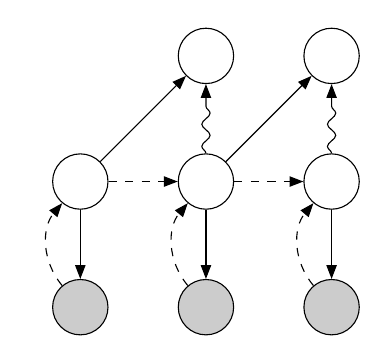
\begin{tikzpicture}[
  node distance=2.5em, auto,
  lat/.style={draw=black, circle, minimum size=2em},
  obs/.style={circle, draw=black, fill=black!20, minimum size=2em},
  gen/.style={->, -{Stealth[length=.5em, inset=0pt]}},
  inf/.style={dashed, ->, -{Stealth[length=.5em, inset=0pt]}},
  div/.style={decorate, decoration={snake, amplitude=.15em, segment length=.8em, post length=.45em}, ->, -{Stealth[length=.5em, inset=0pt]}},
]
\node[obs, inner sep=.02em] (o1) {};
\node[obs, right=of o1, inner sep=.02em] (o2) {};
\node[obs, right=of o2, inner sep=.02em] (o3) {};
\node[lat, above=of o1] (q11) {};
\node[lat, above=of o2] (q22) {};
\node[lat, above=of o3] (q33) {};
\node[lat, above=of q22] (q21) {};
\node[lat, above=of q33] (q32) {};
\path (q11) edge[gen] node {} (o1);
\path (q22) edge[gen] node {} (o2);
\path (q33) edge[gen] node {} (o3);
\path (q11) edge[gen] node {} (q21);
\path (q22) edge[gen] node {} (q32);
\path (o1) edge[inf, bend left=40] node {} (q11);
\path (o2) edge[inf, bend left=40] node {} (q22);
\path (o3) edge[inf, bend left=40] node {} (q33);
\path (q11) edge[inf] node {} (q22);
\path (q22) edge[inf] node {} (q33);
\path (q22) edge[div] node {} (q21);
\path (q33) edge[div] node {} (q32);
\end{tikzpicture}}
\caption{Standard variational bound}
\label{fig:elbo}
\end{subfigure}\hfil \begin{subfigure}[t]{.27\textwidth}
\centering
\scalebox{0.7}{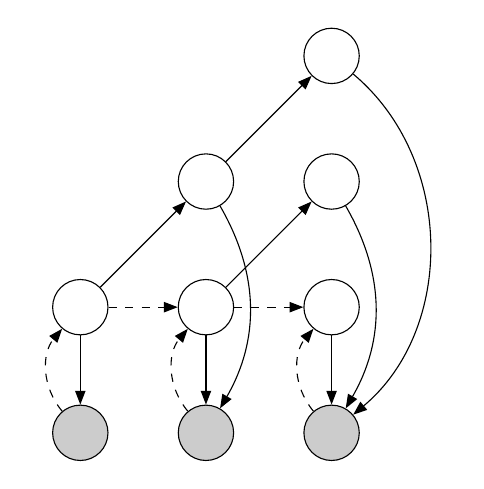
\begin{tikzpicture}[
  node distance=2.5em, auto,
  lat/.style={draw=black, circle, minimum size=2em},
  obs/.style={circle, draw=black, fill=black!20, minimum size=2em},
  gen/.style={->, -{Stealth[length=.5em, inset=0pt]}},
  inf/.style={dashed, ->, -{Stealth[length=.5em, inset=0pt]}},
  div/.style={decorate, decoration={snake, amplitude=.15em, segment length=.8em, post length=.45em}, ->, -{Stealth[length=.5em, inset=0pt]}},
]
\node[obs, inner sep=.02em] (o1) {};
\node[obs, right=of o1, inner sep=.02em] (o2) {};
\node[obs, right=of o2, inner sep=.02em] (o3) {};
\node[lat, above=of o1] (q11) {};
\node[lat, above=of o2] (q22) {};
\node[lat, above=of o3] (q33) {};
\node[lat, above=of q22] (q21) {};
\node[lat, above=of q33] (q32) {};
\node[lat, above=of q32] (q31) {};
\path (q11) edge[gen] node {} (o1);
\path (q22) edge[gen] node {} (o2);
\path (q33) edge[gen] node {} (o3);
\path (q11) edge[gen] node {} (q21);
\path (q22) edge[gen] node {} (q32);
\path (q21) edge[gen] node {} (q31);
\path (q21) edge[gen, bend left=30] node {} (o2);
\path (q32) edge[gen, bend left=30] node {} (o3);
\path (q31) edge[gen, bend left=50] node {} (o3);
\path (o1) edge[inf, bend left=40] node {} (q11);
\path (o2) edge[inf, bend left=40] node {} (q22);
\path (o3) edge[inf, bend left=40] node {} (q33);
\path (q11) edge[inf] node {} (q22);
\path (q22) edge[inf] node {} (q33);
\end{tikzpicture}}
\caption{Observation overshooting}
\label{fig:obsov}
\end{subfigure}\hfil \begin{subfigure}[t]{.27\textwidth}
\centering
\scalebox{0.7}{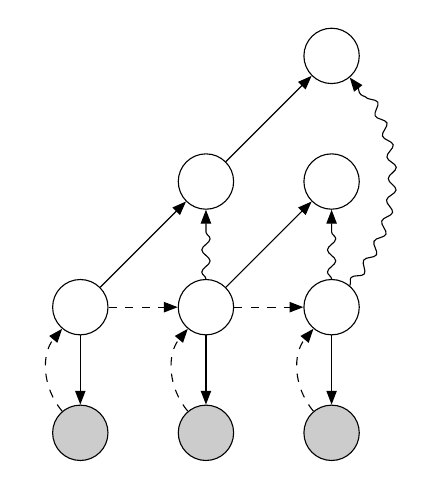
\begin{tikzpicture}[
  node distance=2.5em, auto,
  lat/.style={draw=black, circle, minimum size=2em},
  obs/.style={circle, draw=black, fill=black!20, minimum size=2em},
  gen/.style={->, -{Stealth[length=.5em, inset=0pt]}},
  inf/.style={dashed, ->, -{Stealth[length=.5em, inset=0pt]}},
  div/.style={decorate, decoration={snake, amplitude=.15em, segment length=.8em, post length=.45em}, ->, -{Stealth[length=.5em, inset=0pt]}},
]
\node[obs, inner sep=.02em] (o1) {};
\node[obs, right=of o1, inner sep=.02em] (o2) {};
\node[obs, right=of o2, inner sep=.02em] (o3) {};
\node[lat, above=of o1] (q11) {};
\node[lat, above=of o2] (q22) {};
\node[lat, above=of o3] (q33) {};
\node[lat, above=of q22] (q21) {};
\node[lat, above=of q33] (q32) {};
\node[lat, above=of q32] (q31) {};
\path (q11) edge[gen] node {} (o1);
\path (q22) edge[gen] node {} (o2);
\path (q33) edge[gen] node {} (o3);
\path (q11) edge[gen] node {} (q21);
\path (q22) edge[gen] node {} (q32);
\path (q21) edge[gen] node {} (q31);
\path (o1) edge[inf, bend left=40] node {} (q11);
\path (o2) edge[inf, bend left=40] node {} (q22);
\path (o3) edge[inf, bend left=40] node {} (q33);
\path (q11) edge[inf] node {} (q22);
\path (q22) edge[inf] node {} (q33);
\path (q22) edge[div] node {} (q21);
\path (q33) edge[div] node {} (q32);
\path (q33) edge[div, bend right=40] node {} (q31);
\end{tikzpicture}}
\caption{Latent overshooting}
\label{fig:latov}
\end{subfigure}\hfil\hfil \caption{Unrolling schemes.
The labels  are short for the state at time  conditioned on observations up to time .
Arrows pointing at shaded circles indicate log-likelihood loss terms. Wavy arrows indicate KL-divergence loss terms.
(a) The standard variational objectives decodes the posterior at every step to compute the reconstruction loss. It also places a KL on the prior and posterior at every step, which trains the transition function for one-step predictions.
(b) Observation overshooting \citep{amos2018awareness} decodes all multi-step predictions to apply additional reconstruction losses. This is typically too expensive in image domains.
(c) Latent overshooting predicts all multi-step priors. These state beliefs are trained towards their corresponding posteriors in latent space to encourage accurate multi-step predictions.}
\label{fig:overshooting}
\end{figure*}
 
In the previous section, we derived the typical variational bound for learning and inference in latent sequence models (\cref{eq:elbo}). As show in \cref{fig:elbo}, this objective function contains reconstruction terms for the observations and KL-divergence regularizers for the approximate posteriors. A limitation of this objective is that the stochastic path of the transition function  is only trained via the KL-divergence regularizers for one-step predictions: the gradient flows through  directly into  but never traverses a chain of multiple . In this section, we generalize this variational bound to \emph{latent overshooting}, which trains all multi-step predictions in latent space. We found that several dynamics models benefit from latent overshooting, although our final agent using the RSSM model does not require it (see \cref{sec:exp_overshooting}).

\paragraph{Limited capacity}

If we could train our model to make perfect one-step predictions, it would also make perfect multi-step predictions, so this would not be a problem. However, when using a model with limited capacity and restricted distributional family, training the model only on one-step predictions until convergence does in general not coincide with the model that is best at multi-step predictions. For successful planning, we need accurate multi-step predictions. Therefore, we take inspiration from \citet{amos2018awareness} and earlier related ideas \citep{krishnan2015deepkalman,lamb2016professor,chiappa2017recurrent}, and train the model on multi-step predictions of all distances. We develop this idea for latent sequence models, showing that multi-step predictions can be improved by a loss in latent space, without having to generate additional images.

\paragraph{Multi-step prediction}

We start by generalizing the standard variational bound (\cref{eq:elbo}) from training one-step predictions to training multi-step predictions of a fixed distance . For ease of notation, we omit actions in the conditioning set here; every distribution over  is conditioned upon . We first define multi-step predictions, which are computed by repeatedly applying the transition model and integrating out the intermediate states,
The case  recovers the one-step transitions used in the original model. Given this definition of a multi-step prediction, we generalize \cref{eq:elbo} to the variational bound on the multi-step predictive distribution ,
-2ex]
&\geq\sum_{t=1}^T \Big(
  \describe{\E{\q(s_t|o_{\leq t})}{\ln\p(o_t|s_t)}}{reconstruction} \eqbr&\quad
  -\describe{\Ebelow[\big]{\p(s_{t-1}|s_{t-d})\q(s_{t-d}|o_{\leq t-d})}{\KL{\q(s_t|o_{\leq t})}{\p(s_t|s_{t-1})}}}{multi-step prediction} \Big).
\end{aligned}
\label{eq:dstep}

\frac{1}{D}\sum_{d=1}^D\ln\pr[p_d](o_{1:T}) \geq
\sum_{t=1}^T \Big(
  \describe{\E{\q(s_t|o_{\leq t})}{\ln\p(o_t|s_t)}}{reconstruction} \eqbr
  -\describe{\frac{1}{D}\sum_{d=1}^D
    \beta_d\Ebelow[\big]{\p(s_{t-1}|s_{t-d})\q(s_{t-d}|o_{\leq t-d})}{\KL{\q(s_t|o_{\leq t})}{\p(s_t|s_{t-1})}}}{latent overshooting} \Big).
\label{eq:latov}

\begin{aligned}
\ln\p(o_{1:T}|a_{1:T})
&\triangleq\ln\E[\bigg]{\p(s_{1:T}|a_{1:T})}{\prod_{t=1}^T \p(o_t|s_t)} \\
&=\ln\E[\bigg]{\q(s_{1:T}|o_{1:T},a_{1:T})}{\prod_{t=1}^T \p(o_t|s_t)\p(s_t|s_{t-1},a_{t-1})/\q(s_t|o_{\leq t},a_{<t})} \\
&\geq\E[\bigg]{\q(s_{1:T}|o_{1:T},a_{1:T})}{\sum_{t=1}^T \ln\p(o_t|s_t)+\ln\p(s_t|s_{t-1},a_{t-1})-\ln\q(s_t|o_{\leq t},a_{<t})} \\
&=\sum_{t=1}^T \Big(
  \describe{\Ebelow{\q(s_t|o_{\leq t},a_{<t})}{\ln\p(o_t|s_t)}}{reconstruction}
  -\describe{\Ebelow[\big]{\q(s_{t-1|o_{\leq t-1},a_{<a-1}})}{\KL{\q(s_t|o_{\leq t},a_{<t})}{\p(s_t|s_{t-1},a_{t-1})}}}{complexity} \Big).
\end{aligned}
\label{eq:elbo_deriv}

\begin{aligned}
\ln\pr[p_d](o_{1:T}|a_{1:T})
&\triangleq\ln\E[\bigg]{\pr[p_d](s_{1:T}|a_{1:T})}{\prod_{t=1}^T\p(o_t|s_t)} \\
&=\ln\E[\bigg]{\q(s_{1:T}|o_{1:T},a_{1:T})}{\prod_{t=1}^T \p(o_t|s_t)\p(s_t|s_{t-d},a_{t-d-1:t-1})/\q(s_t|o_{\leq t},a_{<t})} \\
&\geq\E[\bigg]{\q(s_{1:T}|o_{1:T},a_{1:T})}{\sum_{t=1}^T \ln\p(o_t|s_t)+\ln\p(s_t|s_{t-d},a_{t-d-1:t-1})-\ln\q(s_t|o_{\leq t},a_{<t})} \\
&\geq\E[\bigg]{\q(s_{1:T}|o_{1:T},a_{1:T})}{\sum_{t=1}^T \ln\p(o_t|s_t)+\Ebelow{\p(s_{t-1}|s_{t-d},a_{t-d-1:t-2})}{\ln\p(s_t|s_{t-1},a_{t-1})}-\ln\q(s_t|o_{\leq t},a_{<t})} \\
&=\sum_{t=1}^T \Big(
  \describe{\E{\q(s_t|o_{\leq t},a_{<t})}{\ln\p(o_t|s_t)}}{reconstruction}
  -\describe{\Ebelow[\big]{\p(s_{t-1}|s_{t-d},a_{t-d-1:t-2})\q(s_{t-d}|o_{\leq t-d},a_{<t-d})}{\KL{\q(s_t|o_{\leq t},a_{<t})}{\p(s_t|s_{t-1},a_{t-1})}}}{multi-step prediction} \Big).
\end{aligned}
\label{eq:dstep_deriv}

\begin{aligned}
\MI{s_t;s_{t-d}} &\leq \MI{s_t;s_{t-1}} \\
\H{s_t}-\H{s_t|s_{t-d}} &\leq \H{s_t}-\H{s_t|s_{t-1}} \\
\E{}{\ln\p(s_t|s_{t-d})} &\leq \E{}{\ln\p(s_t|s_{t-1})} \\
\E{}{\ln\pr[p_d](o_{1:T})} &\leq \E{}{\ln\p(o_{1:T})}.
\end{aligned}
\label{eq:dataproc_deriv}

Therefore, any bound on the multi-step predictive distribution, including \cref{eq:dstep_deriv} and \cref{eq:latov}, is also a bound on the one-step predictive distribution.

\clearpage
\section{Additional Related Work}
\label{sec:more_related_work}

\paragraph{Planning in state space}

When low-dimensional states of the environment are available to the agent, it is possible to learn the dynamics directly in state space. In the regime of control tasks with only a few state variables, such as the cart pole and mountain car tasks, PILCO \citep{deisenroth2011pilco} achieves remarkable sample efficiency using Gaussian processes to model the dynamics. Similar approaches using neural networks dynamics models can solve two-link balancing problems \citep{gal2016deeppilco,higuera2018synthesizing} and implement planning via gradients \citep{henaff2018planbybackprop}. \citet{chua2018pets} use ensembles of neural networks, scaling up to the cheetah running task. The limitation of these methods is that they access the low-dimensional Markovian state of the underlying system and sometimes the reward function. \citet{amos2018awareness} train a deterministic model using overshooting in observation space for active exploration with a robotics hand. We move beyond low-dimensional state representations and use a latent dynamics model to solve control tasks from images.

\paragraph{Hybrid agents}

The challenges of model-based RL have motivated the research community to develop hybrid agents that accelerate policy learning by training on imagined experience \citep{kalweit2017blending,nagabandi2017mbmf,kurutach2018modeltrpo,buckman2018steve,ha2018worldmodels}, improving feature representations \citep{wayne2018merlin,igl2018dvrl}, or leveraging the information content of the model directly \citep{weber2017i2a}. \citet{srinivas2018upn} learn a policy network with integrated planning computation using reinforcement learning and without prediction loss, yet require expert demonstrations for training.

\paragraph{Multi-step predictions}

Training sequence models on multi-step predictions has been explored for several years. Scheduled sampling \citep{bengio2015scheduled} changes the rollout distance of the sequence model over the course of training. Hallucinated replay \citep{talvitie2014hallucinated} mixes predictions into the data set to indirectly train multi-step predictions. \citet{venkatraman2015dad} take an imitation learning approach. Recently, \citet{amos2018awareness} train a dynamics model on all multi-step predictions at once. We generalize this idea to latent sequence models trained via variational inference.

\paragraph{Latent sequence models}

Classic work has explored models for non-Markovian observation sequences, including recurrent neural networks (RNNs) with deterministic hidden state and probabilistic state-space models (SSMs). The ideas behind variational autoencoders \citep{kingma2013vae,rezende2014vae} have enabled non-linear SSMs that are trained via variational inference \citep{krishnan2015deepkalman}. The VRNN \citep{chung2015vrnn} combines RNNs and SSMs and is trained via variational inference. In contrast to our RSSM, it feeds generated observations back into the model which makes forward predictions expensive. \citet{karl2016dvbf} address mode collapse to a single future by restricting the transition function, \citep{moerland2017learning} focus on multi-modal transitions, and \citet{doerr2018prssm} stabilize training of purely stochastic models. \citet{buesing2018dssm} propose a model similar to ours but use in a hybrid agent instead for explicit planning.

\paragraph{Video prediction}

Video prediction is an active area of research in deep learning. \citet{oh2015atari} and \citet{chiappa2017recurrent} achieve visually plausible predictions on Atari games using deterministic models. \citet{kalchbrenner2016vpn} introduce an autoregressive video prediction model using gated CNNs and LSTMs. Recent approaches introduce stochasticity to the model to capture multiple futures \citep{babaeizadeh2017sv2p,denton2018stochastic}. To obtain realistic predictions, \citet{mathieu2015deep} and \citet{vondrick2016generating} use adversarial losses. In simulated environments, \citet{gemici2017temporalmemory} augment dynamics models with an external memory to remember long-time contexts. \citet{van2017vq} propose a variational model that avoids sampling using a nearest neighbor look-up, yielding high fidelity image predictions. These models are complimentary to our approach.

\clearpage
\section{Video Predictions}
\label{sec:prediction}
\begin{figure*}[h]
\providecommand{\width}{}
\renewcommand{\width}{0.62\textwidth}
\centering
\begin{subfigure}[t]{\width}
\rot{\hspace{4.6em}\method}
\hspace{.5em}
\includegraphics[width=\textwidth]{prediction/cheetah-planet}
\end{subfigure} \\
\vspace{2ex}
\begin{subfigure}[t]{\width}
\rot{\hspace{1.3em}\method + Overshooting}
\hspace{.5em}
\includegraphics[width=\textwidth]{prediction/cheetah-latov}
\end{subfigure} \\
\vspace{2ex}
\begin{subfigure}[t]{\width}
\rot{\hspace{1.8em}Deterministic (GRU)}
\hspace{.5em}
\includegraphics[width=\textwidth]{prediction/cheetah-rnn}
\end{subfigure} \\
\vspace{2ex}
\begin{subfigure}[t]{\width}
\rot{\hspace{2.5em}Stochastic (SSM)}
\hspace{.5em}
\includegraphics[width=\textwidth]{prediction/cheetah-ssm}
\end{subfigure} \\
\caption{Open-loop video predictions for test episodes. The \mbox{columns 1--5} show reconstructed context frames and the remaining images are generated open-loop. Our RSSM achieves pixel-accurate predictions for 50 steps into the future in the cheetah environment. We randomly selected action sequences from test episodes collected with action noise alongside the training episodes.}
\label{fig:prediction}
\vspace{-0.2in}
\end{figure*} 
\clearpage
\section{State Diagnostics}

\begin{figure}[h]
\centering
\includegraphics[width=\textwidth]{diagnostics/diagnostics}
\caption{Open-loop state diagnostics. We freeze the dynamics model of a \method agent and learn small neural networks to predict the true positions, velocities, and reward of the simulator. The open-loop predictions of these quantities show that most information about the underlying system is present in the learned latent space and can be accurately predicted forward further than the planning horizons used in this work.}
\label{fig:diagnostics}
\end{figure} 
\clearpage
\section{Planning Parameters}

\begin{figure}[h!]
\centering
\includegraphics[width=\textwidth]{figures/mpc/mpc}
\caption{Planning performance on the cheetah running task with the true simulator using different planner settings. Performance ranges from 132 (blue) to 837 (yellow). Evaluating more action sequences, optimizing for more iterations, and re-fitting to fewer of the best proposals tend to improve performance. A planning horizon length of 6 is not sufficient and results in poor performance. Much longer planning horizons hurt performance because of the increased search space. For this environment, best planning horizon length is near 8 steps.}
\end{figure}  
\end{document}
